\section{Introduction}
Multi-modal data fusion is a ubiquitous problem in signal processing and machine
learning. In many applications, we have access to multiple datasets, possibly of different
modalities, each of which describe some feature of the system. This setup is becoming
increasingly common today as data collection becomes cheaper and easier. We are no longer
limited by the amount or variety of data that we can collect, but instead by how quickly
and accurately we can process such a wide variety of data. Access to more
than two datasets arises in applications such as handwritten digit classification
\cite{yu2007learning}, multi-temporal hyperspectral imaging \cite{nielsen2002multiset},
and medical imaging \cite{correa2010canonical, deleus2011functional}.

Unlike the two dataset case, there is not a singular definition for correlation between
more than two random variables. Kettenring \cite{kettenring1971canonical} considers five
such definitions that extend Hotellings's \cite{hotelling1936relations} original canonical
correlation analysis (CCA) work. These five formulations of multiset CCA (MCCA) unify
multiset correlation analysis of the previous decades \cite{vinograde1950canonical,
  steel1951minimum, horst1961relations, horst1961generalized}. Nielsen
\cite{nielsen1994analysis} later extended Kettenring's analysis by also considering four
constraint functions placed on the canonical vectors in the optimization problem.

In this paper consider the performance of one MCCA optimization problem, MAXVAR. We show
that, similar to empirical CCA, the solution to this problem is a SVD of a matrix with block
entries of the pairwise product of right singular vectors of the individual datasets. We
then apply the same principles used in informative CCA (ICCA) to develop an informative version of MAXVAR,
which we call IMCCA. Using the idea of trim-then-fuse, we propose to trim all data SVDs to
include only the \textit{informative} singular vectors. We provide some analysis of the
behavior of these algorithms and provide a test statistic to use to determine the number
of correlations present in multiple datasets. We discuss why multi-dataset correlation
analysis is difficult but showcase on a real world dataset that IMCCA greatly outperforms
MAXVAR and can robustly identify sources of correlation.


\section{Mathematical Formulation of MCCA}

Let $y_1,y_2,\dots,y_m$ be observations drawn from $m$ distributions $y_i\sim
\mathcal{Y}_i$ with $y_i\in\complex^{d_i}$. Assume, without loss of generality, that $y_i$
is zero mean. Define the covariance between distributions as $\E{y_iy_j^T}=R_{ij}$ for
$i,j=1,\dots,m$. Define the joint observation vector $y$ and its covariance $R=\E{yy^H}$ as
\be
y = \left[\begin{array}{c}y_1\\ \vdots \\ y_m\end{array}\right] \in\complex^{d\times 1},\,\,\,\,R
= \left[\begin{array}{ccc}R_{11}&\dots&R_{1m}\\ \vdots&\ddots&\vdots\\ 
    R_{m1}&\dots&R_{mm}\end{array}\right]\in\complex^{d\times d}
\ee
where $d=\sum_{i=1}^md_i$.

The goal of MCCA is to find canonical coefficient vectors, $x_i\in\complex^{d_i\times 1}$
for $i=1,\dots,m$, such that the canonical variates, $w_i=x_i^Hy_i$, are optimal with
respect to an objective function $J(\cdot)$ and constraint function $h(\cdot)$. Define the
vector of canonical vectors as 
$x=\left[x_1^H,\dots,x_m^H\right]^H\in\complex^{d\times 1}$ and the vector of canonical
variates as $w=[w_1,\dots,w_m]^H\in\complex^{m\times 1}$. The covariance matrix of $w$ is
\begin{equation*}
\Phi(x)=\E{ww^H}=\left[\begin{array}{ccc} x_1^HR_{11}x_1 & \dots & x_1^HR_{1m}x_m \\ \vdots
    & \ddots & \vdots \\ x_m^HR_{m1}x_1 & \dots & x_m^HR_{mm}x_m\\ \end{array}\right].
\end{equation*}
Using this notation, the MCCA optimization problem is
\begin{equation}\label{eq:chpt10:opt_prob}
\begin{aligned}
&\underset{x}{\mathop{\rm optimize}} && J(\Phi(x))\\
&\text{subject to} && h(x,R).\\
\end{aligned}
\end{equation}
For this paper we consider the maximum variance (MAXVAR) objective function with the
constraint functions
  \begin{equation*}
    x_i^HR_{ii}x_i = 1,\, 1\leq i\leq m,
  \end{equation*}
which require the canonical variate to be unit norm.

\subsection{Solution to MAXVAR}
The MAXVAR optimization problem is
\begin{equation*}
\begin{aligned}
&\argmax_{x}&&\lambda\\
&\text{s.t.} &&x_i^HR_{ii}x_i  = 1\,\,,1\leq i\leq m\\
&&& \Phi(x) a = \lambda a\\
&&& a^Ha=1.\\
\end{aligned}
\end{equation*}
Writing $\Phi(x) = X^H R X$, where $X=\blkdiag(x_1,\dots,x_m)$, and making the
transformation $\widetilde{a}=R_D^{1/2}Xa$, where $R_D=\blkdiag(R_{11},\dots,R_{mm})$,
this optimization problem becomes.
\begin{equation*}
\begin{aligned}
&\argmax_{\widetilde{a}}&&\lambda\\
&\text{s.t}&& \widetilde{a}^HR_D^{-1/2}RR_D^{-1/2}\widetilde{a} = \lambda\\
&&& \widetilde{a}^H\widetilde{a}=1.\\
\end{aligned}
\end{equation*}
Our canonical vectors are found by inverting the transformation 
\be
x_i = \frac{R_{ii}^{-1/2}\widetilde{a}_i}{\|\widetilde{a}_i\|},
\ee
where $\widetilde{a}_i\in\complex^{d_i}$ is the component of $\widetilde{a}$ corresponding
to dataset $i$.

\subsection{Empirical MAXVAR}

In many real-world applications, the covariance matrices used to form $R$ and $R_D$ are
unknown and estimated from training data matrices $Y_1=\left[y_1^{(1)},\dots
  y_1^{(n)}\right]\in\complex^{d_1\times n},\dots, Y_m=\left[y_m^{(1)},\dots,
  y_m^{(n)}\right]\in\complex^{d_m\times n}$. We denote the SVD of each training dataset
as $Y_i=U_i\Sigma_iV_i^H$ and form the matrices $U\in\complex^{d\times
  d}=\blkdiag(U_1,\dots,U_m)$, $\Sigma\in\complex^{d\times
  nm}=\blkdiag(\Sigma_1,\dots,\Sigma_m)$, and $V\in\complex^{n\times nm}=[V_1,\dots,V_m]$.
Using these data SVDs, we form sample covariance matrices,
$\widehat{R}_{ij}=\frac{1}{n}Y_iY_j^H = \frac{1}{n}U_i\Sigma_iV_i^HV_j\Sigma_j^HU_j^H$
with which we form $\widehat{R}=U\Sigma V^HV\Sigma^HU^H$ and
$\widehat{R}_D=U\Sigma\Sigma^HU^H$.

Our empirical eigen-system is
$\widehat{R}_D^{-1/2}\widehat{R}\widehat{R}_D^{-1/2}\widetilde{a} =
\widehat{\rho}\widetilde{a}$. Using the SVD notation for our empirical data matrices, we
have that
\begin{equation*}
\begin{aligned}
&\widehat{R}_D^{-1/2}\widehat{R}\widehat{R}_D^{-1/2}&&=\left(U\Sigma\Sigma^HU^H\right)^{-1/2}\left(U\Sigma V^HV\Sigma^H U^H\right)\left(U\Sigma\Sigma^HU^H\right)^{-1/2}\\
&&&=U(\Sigma\Sigma^H)^{-1/2}U^HU\Sigma V^HV\Sigma^HU^HU(\Sigma\Sigma^H)^{-1/2}U^H\\
&&& = U(\Sigma\Sigma^H)^{-1/2}\Sigma V^HV\Sigma^H(\Sigma\Sigma^H)^{-1/2}U^H\\
&&&=U\widetilde{V}^H\widetilde{V}U^H
\end{aligned}
\end{equation*}
where $\tilde{V}\in\complex^{n\times d}=[V_1(:,1:d_1),\dots,V_m(:,1:d_m)]$. Defining $\widehat{C} = \widetilde{V}^H\widetilde{V}$ and its eigenvalue decomposition $\widehat{C} = \widehat{F}\widehat{K}\widehat{F}^H$, then we have that the MCCA empirical solution is
\be\ba
& \widehat{\rho} = \widehat{k}_1\\
& \widehat{x} = U \widetilde{\Sigma}^{-1}\Lambda_{\widehat{f}_1}^{-1}\widehat{f}_1
\ea\ee
where $\widetilde{\Sigma} = \blkdiag\left(\Sigma_1(1:d_1,1:d_1),\dots, \Sigma_m(1:d_m,1:d_m)\right)$.

\section{Proposed Informative MCCA Algorithm}

In the above derivations, we saw the importance of the matrix
$\Rmcca=R_D^{-1/2}RR_D^{-1/2}$. Importantly, we see that the rank of $\Rmcca$ is exactly
equal to the number of correlated components in our datasets. However, in practical
application we must estimate this matrix using training data. The singular values of
$\widehat{C}_{\text{mcca}}$ have the same singular values as
\beq\label{eq:chpt10:R_mcca}
\Rmccahat =
\left[\begin{array}{c}V_1^H\\V_2^H\\\vdots\\V_m^H\end{array}\right]\left[\begin{array}{cccc}V_1
    & V_2 & \cdots & V_m\end{array}\right] = \left[\begin{array}{cccc}I_{d_1} & 
    V_1^HV_2 & \cdots & V_1^HV_m\\ V_2^HV_1 & I_{d_2}& \cdots & V_2^HV_m\\
  \vdots & \vdots & \ddots & \vdots \\ V_m^HV_1 & V_m^HV_2 & \cdots & I_{d_m}\end{array}\right].
\eeq
Motivated by the results in \cite{pezeshki2004empirical}, we expect that in the sample
deficient regime, the eigenvalues of $\Rmccahat$ will not be able to reliably detect
correlations between multiple datasets. We provide the following results about the
eigenvalues of $\Rmccahat$.

\begin{Th}\label{th:maxvar}
If $2n<\min_{i\neq j\neq k}(d_i+d_j+d_k)$ then the largest eigenvalue of $\Rmccahat$ is equal
to $m$. 
\end{Th}

\begin{Th}\label{th:minvar}
If $n<\sum_{i=1}^md_i$ then the smallest eigenvalue of $\Rmccahat$ is zero.
\end{Th}

\begin{Conj}\label{conj:minmaxvar}
We conjecture that when $n<\sum_{i=1}^md_i$, the largest eigenvalue of $\Rmccahat$ is
determined entirely based on $n$ and $\sum_{i=1}^md_i$ and not on the underlying
correlation.
\end{Conj}

Theorem \ref{th:maxvar} states that in a certain sample deficient regime, the largest
eigenvalues of $\Rmccahat$ are deterministic. Similarly, Theorem \ref{th:minvar} states that
in a different sample deficient regime, the smallest eigenvalues are deterministically
zero. These sample deficient regimes are different for the largest and smallest
eigenvalues; the regime is larger for the smaller eigenvalues. Conjecture
\ref{conj:minmaxvar} bridges this gap. The intuition is based on the observation from
\cite{bach2003kernel} that in the two dataset case of CCA, the eigenvalues of $\Rmccahat$ come in pairs $\left\{1+k_i,1-k_i\right\}$. When there are more than two datasets, we believe that the
eigenvalues of $\Rmccahat$ are still coupled. Therefore, due to the hypothesized coupling of the largest and smallest
eigenvalues we believe Conjecture \ref{conj:minmaxvar} holds. In this setting, like in
empirical CCA, we conjecture that the canonical vectors are simply random and we would not
like to use them in an algorithm.

\subsection{Informative MCCA}

As evident in the theorems above, in the sample deficient regime we cannot analyze the
rank of $\Rmccahat$ to determine the number of correlated components existing in our
datasets. In this regime, the eigenvalues of $\Rmccahat$ are deterministic, regardless of
whether a correlated signal is present. Recalling (\ref{eq:chpt10:R_mcca}), we observe
that $\Rmccahat$ uses all right singular values of every dataset. When modeling each
data matrix as a low-rank signal matrix plus noise, we know that not all right singular
vectors are informative. In the spirit of the ICCA algorithm
\cite{nadakuditi2011fundamental} and motivated by the ubiquitous low-rank
signal-plus-noise data models in signal processing, we propose to first trim our data
matrices
\be\ba
& \Ucir_j = \widehat{U}_j\left(:,1:\widehat{k}_j\right),&& \Vcir_j = \widehat{V}_j\left(:,1:\widehat{k}_j\right),
\ea\ee
where $\widehat{k}_j$ for $j=1,\dots,m$ are estimates of the number of signals present in
each dataset. Using these trimmed data matrices, we create the low rank matrices
\be
\Ucir = \blkdiag(\Ucir_1,\dots,\Ucir_m),\,\,\,\,\Vcir =
\left[\Vcir_1,\dots \Vcir_m\right] .
\ee
Using these trimmed estimates, we define the informative MAXVAR (IMCCA) matrix as
\be
\Rmccatil = \Ucir\Vcir^H\Vcir\Ucir^H.
\ee
We then use this matrix in the MAXVAR algorithm to retrieve correlation estimates and
canonical vector estimates. 

\section{Video-Video-Video Experiment}

To verify the effectiveness of IMCCA for real world applications and to showcase the
extreme sub-optimality of empirical MCCA, we setup a controlled experiment consisting of
four stationary flashing lights and three stationary iPhone cameras. Figure
\ref{fig:chpt10:mcca_sources} shows the left, middle, and right camera views for one frame
of the video experiment and manually identifies each source in each camera view by drawing
a colored box around it. All cameras share the red boxed source. The left and right views
share the green boxed source. The left and right views also each have an independent
source in their view.

\begin{figure}
  \begin{center}
    \subfigure[Left Camera]{
      \label{fig:chpt10:mcca_man_left}
      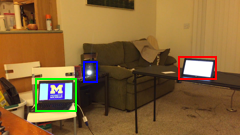
\includegraphics[width=0.3\textwidth]{chpt10_mcca/figs/mcca_left_man.png}
    }
    \subfigure[Middle Camera]{
      \label{fig:chpt10:mcca_man_mid}
      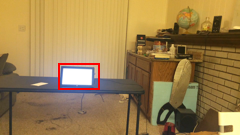
\includegraphics[width=0.3\textwidth]{chpt10_mcca/figs/mcca_mid_man.png}
    }
    \subfigure[Right Camera]{
      \label{fig:chpt10:mcca_man_right}
      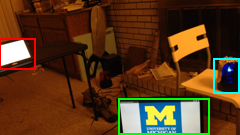
\includegraphics[width=0.3\textwidth]{chpt10_mcca/figs/mcca_right_man.png}
    }   
    \caption{Manual identification of each source in each camera. All three sources share
      a common flashing tablet, outlined in red. The left and right camera views share a
      common flashing laptop screen, outlined in green. The left camera has an independent
      flashing phone light, outlined in dark blue. The right camera has an independent
      flashing police light, outlined in cyan.}
    \label{fig:chpt10:mcca_sources}
  \end{center}
\end{figure}

To synchronize the cameras we used the RecoLive MultiCam iPhone app
\footnote{http://recolive.com/en/}. After turning on all light sources, we recorded 20
seconds of video at 30 frames per second. The resolutions of the iPhone's cameras were all
$1920\times 1080$ pixels. To post-process the video data, we first converted the video
streams to grayscale and then downsampled each spatial dimension by a factor of 8,
resulting in a resolution of $240\times 135$. We then vectorized each image and stacked
the 600 frames into data matrices, all of dimension $32400 \times 600$. 

We run MCCA and IMCCA after every new frame. Specifically, for frame $\ell$, we construct
the $32400\times \ell$ submatrices $Y_{\text{left}}^{\ell}$, $Y_{\text{middle}}^{\ell}$,
and $Y_{\text{right}}^{\ell}$ by taking the matrix of the first $\ell$ original vectorized
frames in each view and then subtracting the mean of the resulting submatrix. We then use
these resulting submatrices as inputs to MCCA and IMCCA. Using our knowledge of the number
of sources in each camera, we set $\widehat{k}_{\text{left}}=3$,
$\widehat{k}_{\text{middle}}=1$, and $\widehat{k}_{\text{right}}=3$. Figure
\ref{fig:chpt10:mcca_corrs} plots the top 3 correlation coefficients returned by MCCA and
IMCCA over the 600 frames of the video. As expected due to our extreme sample deficient
regime, MCCA returns coefficients equal to $2=m-1$, which incorrectly identifies the top
three canonical vectors as being perfectly correlated. IMCCA correctly identifies two
correlations that exist. The third correlation returned by IMCCA is essentially zero.

\begin{figure}
  \begin{center}
    \subfigure[MCCA]{
      \label{fig:chpt10:mcca_mid_u1}
      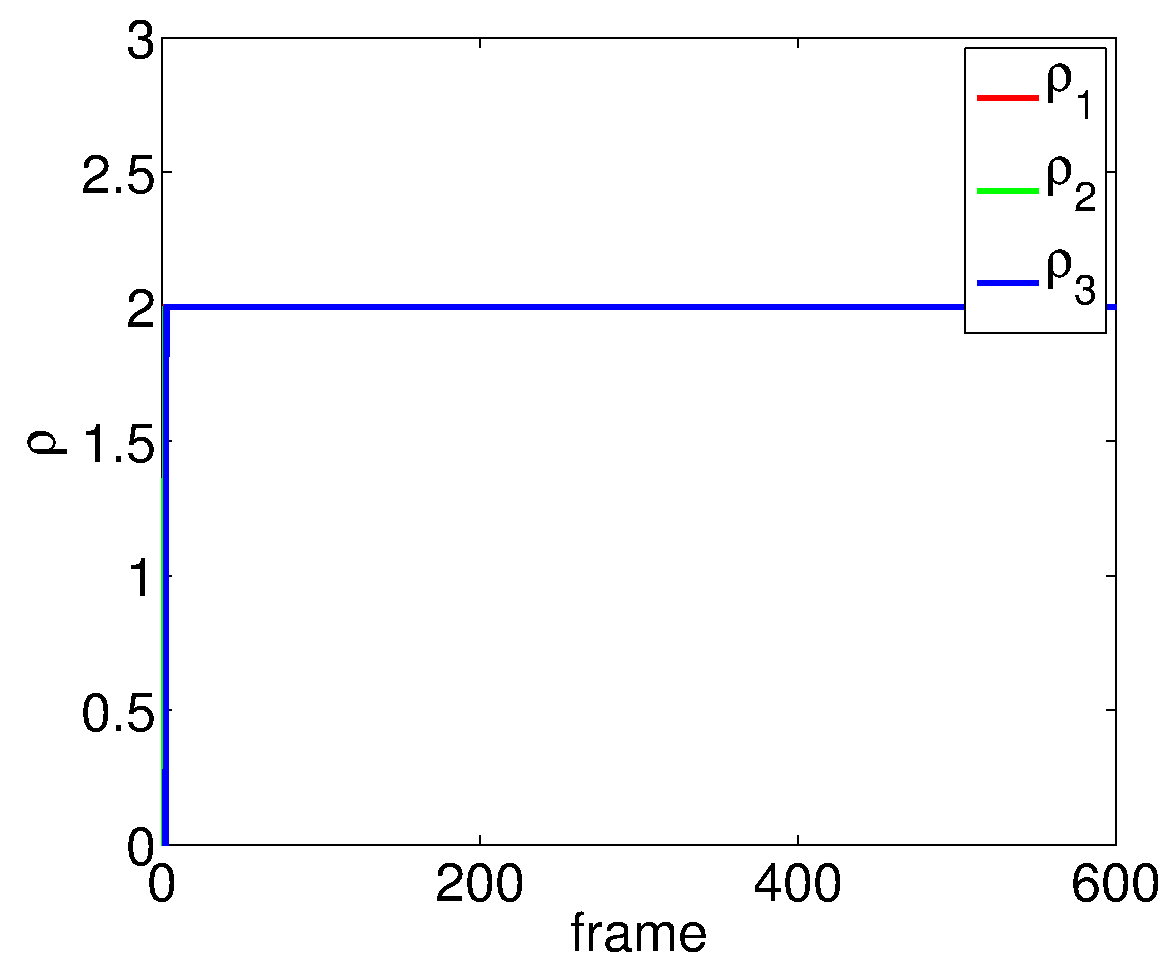
\includegraphics[width=0.4\textwidth]{chpt10_mcca/figs/mcca_cca_corrs.pdf}
    }
    \subfigure[IMCCA]{
      \label{fig:chpt10:mcca_mid_overlay}
      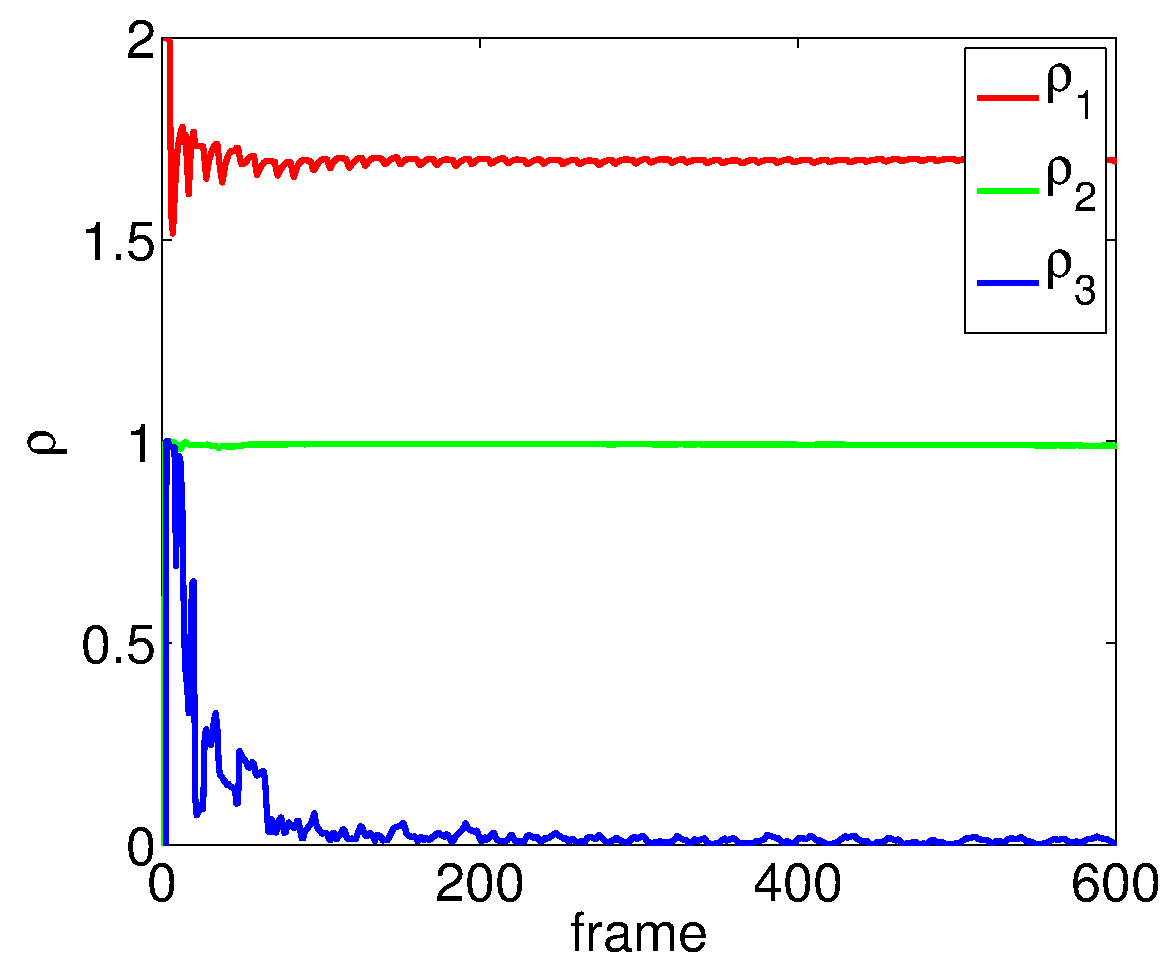
\includegraphics[width=0.4\textwidth]{chpt10_mcca/figs/mcca_icca_corrs.pdf}
    }   
    \caption{Top 3 correlations returned by MCCA and IMCCA.}
    \label{fig:chpt10:mcca_corrs}
  \end{center}
\end{figure}

Figures \ref{fig:chpt10:mcca_cca_vects} and \ref{fig:chpt10:mcca_icca_vects} overlay the
thresholded canonical vectors corresponding to the correlations in Figure
\ref{fig:chpt10:mcca_corrs} onto the original scene for MCCA and IMCCA,
respectively. Unsurprisingly, the MCCA canonical vectors appear extremely random and noisy
while the IMCCA canonical vectors correctly identify the two sources of correlation in our
video. Additionally, IMCCA identifies that once source of correlation appears in all three
camera views (red pixels) and that one source of correlation appears in only two camera
views (green pixels). To overlay the canonical correlations on the original scene, we use
the following thresholding technique
\begin{enumerate}
\item $\widetilde{u}_i = \sqrt{m}u_i$
\item If $\|\widetilde{u}_i^{(j)}\|_2 >1$, then $\widetilde{u}_i^{(j)} =
  \widetilde{u}_i^{(j)}/\|\widetilde{u}_i^{(j)}\|_2$ for $j=1,\dots,m$
\item Threshold $\widetilde{u}_i^{(j)}$ keeping entries greater than $\sqrt{\log(d_i)/d_i}$
\end{enumerate}

\begin{figure}
  \begin{center}
    \subfigure[Left Camera]{
      \label{fig:chpt10:mcca_cca_left}
      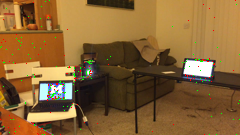
\includegraphics[width=0.3\textwidth]{chpt10_mcca/figs/mcca_left_cca.png}
    }
    \subfigure[Middle Camera]{
      \label{fig:chpt10:mcca_cca_mid}
      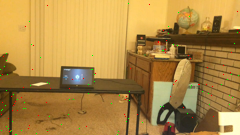
\includegraphics[width=0.3\textwidth]{chpt10_mcca/figs/mcca_mid_cca.png}
    }
    \subfigure[Right Camera]{
      \label{fig:chpt10:mcca_cca_right}
      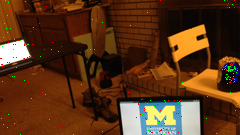
\includegraphics[width=0.3\textwidth]{chpt10_mcca/figs/mcca_right_cca.png}
    }   
    \caption{Top 2 thresholded MCCA canonical vectors overlayed onto the original
      scene. The red pixels are the pixels corresponding to the largest correlation and
      the green pixels correspond to the pixels with the second largest correlation. Since
      we are in the sample deficient regime, MCCA returns random pixels as the canonical
      vectors are random.}
    \label{fig:chpt10:mcca_cca_vects}
  \end{center}
\end{figure}

\begin{figure}
  \begin{center}
    \subfigure[Left Camera]{
      \label{fig:chpt10:mcca_icca_left}
      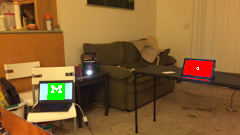
\includegraphics[width=0.3\textwidth]{chpt10_mcca/figs/mcca_left_icca.png}
    }
    \subfigure[Middle Camera]{
      \label{fig:chpt10:mcca_icca_mid}
      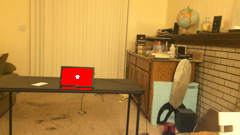
\includegraphics[width=0.3\textwidth]{chpt10_mcca/figs/mcca_mid_icca.png}
    }
    \subfigure[Right Camera]{
      \label{fig:chpt10:mcca_icca_right}
      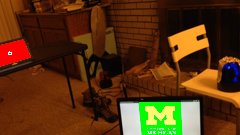
\includegraphics[width=0.3\textwidth]{chpt10_mcca/figs/mcca_right_icca.png}
    }   
    \caption{Top 2 thresholded IMCCA canonical vectors overlayed onto the original
      scene. The red pixels correspond to the largest correlation and the green pixels
      correspond to the second largest correlation. Clearly, the red pixels identify the
      shared flashing tablet light in all 3 views and the green pixels identify the shared
      flashing laptop in the left and right views.}
    \label{fig:chpt10:mcca_icca_vects}
  \end{center}
\end{figure}


